\chapter{Indústria 4.0 e Internet das Coisas}
\label{chapter:industria_4_0_iot}

A revolução dos dados atingiu praticamente todas as áreas de engenharia elétrica, desde a eletrônica, desenvolvendo dispositivos capazes de receber dados telemétricos, processa-los e envia-los para demais hubs, a servidores de armazenamento de dados, recorrentemente chamados de Data Warehouses. Esse conjunto de mudanças engloba a Indústria 4.0, uma indústria que capta dados de suas máquinas em tempo real em larga escala, analisa, armazena, e utiliza inteligência artificial e estatística, para tomada de decisões estratégicas, contando sempre , é claro, com ajustes humanos.

\section{Internet das Coisas}
\label{section:iot}

Dentre o meio da Indústria 4.0, encontra-se a internet das coisas ou IoT, responsável por estruturar as aplicações de aquisição, transmissão e armazenamento de dados a serem analisados. Não é uma surpresa que este setor envolva áreas como eletrônica, computação e telecomunicações em um pacote só. De fato suas camadas são mundos diferentes interligados a um propósito : transmitir dados sobre um dispositivo e/ou para um dispositivo em tempo real.

Pode-se definir IoT como a estrutura que comunica dispositivos em rede, permitindo a transmissão de dados sobre estes em tempo real. É a ponte que permite a troca de informações sobre um dispositivo, qual seu status, seu desempenho, suas condições físicas e do ambiente ao seu redor. Mas, para que este ciclo esteja completo é necessário camadas que desempenham tarefas específicas, para que o dado chegue a quem ou a o que está esperando.

\section{As Camadas do IoT}
\label{section:camadas_iot}

Semelhante as camadas de rede, as camadas de IoT também exercem funções específicas no transporte de dados, e a camada acima não necessariamente precisa saber como a inferior funciona, somente precisa dos dados que esta camada entrega e executar suas tarefas sobre estes até chegar ao destino especificado.

\begin{figure}[h!]
\label{fig:1.1.0/camadas_iot}
\centering
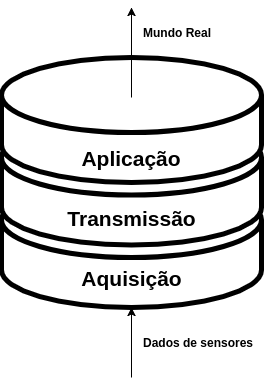
\includegraphics[width=5cm]{./02_Capitulos/02_Cap1/figures/iot_stack}
\caption{As três camadas do IoT, dos sensores ao mundo real}
\end{figure}

A primeira camada é a de aquisição de dados, que lida com o mundo físico e amostra estes dados através de sensores e conversores A/D, também realiza o processamento para entregar em um formato adequado para transmissão e entendível do outro lado, dependo da aplicação. A segunda camada é a camada de transmissão, onde estão, efetivamente, as camadas de rede embutidas. Como o nome já denuncia, ela lida com os aspectos de rede e comunicação para que o dados cheguem as seus destinos. E por último temos a camada de aplicação, a mais abrangente e que envolve maior poder computacional. Ela recebe os dados e lida com os processos de aplicação destes dados, seja análise, visualização, armazenamento ou a estruturação destes.

\subsection{Aquisição}
\label{subsection:aquisicao}



\subsection{Transmissão}
\label{subsection:transmicao}

\subsection{Aplicação}
\label{subsection:aplicacao}



